\documentclass[border=10pt]{standalone}
\usepackage{pgfplots}
\pgfplotsset{compat=1.18}
\begin{document}
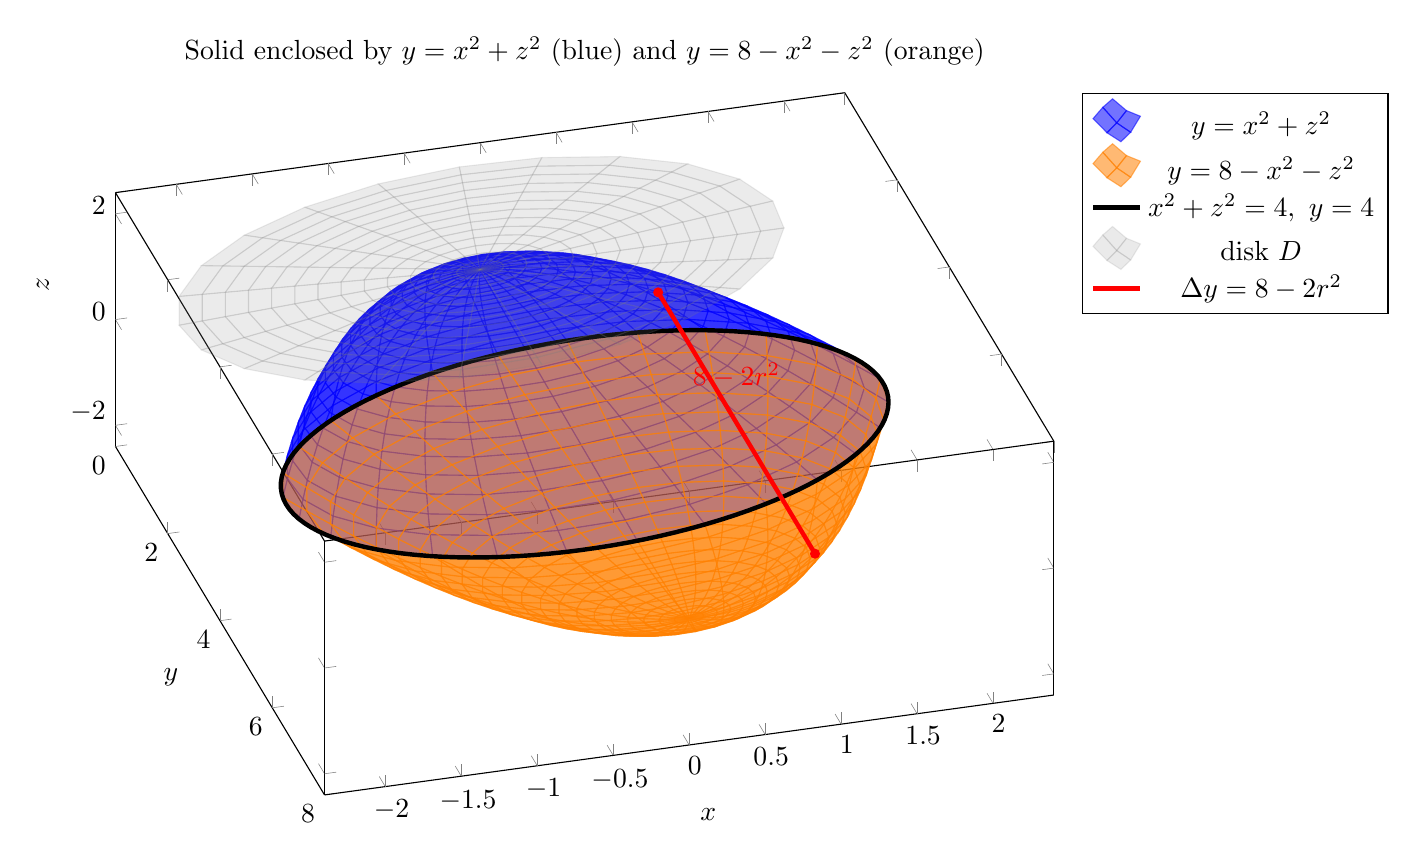
\begin{tikzpicture}
\begin{axis}[
    width=13.5cm, height=10.5cm,
    view={16}{-55},
    xlabel=$x$, ylabel=$y$, zlabel=$z$,
    xmin=-2.4, xmax=2.4, ymin=0, ymax=8, zmin=-2.4, zmax=2.4,
    ztick={-2,0,2}, ytick={0,2,4,6,8},
    title={Solid enclosed by $y=x^2+z^2$ (blue) and $y=8-x^2-z^2$ (orange)},
    legend pos=outer north east,
]
% --- lower paraboloid  y = x^2 + z^2 ---
\addplot3[surf, domain=0:2, domain y=0:360, samples=22, samples y=28,
          blue, opacity=0.55, shader=flat] ({x*cos(y)}, {x^2}, {x*sin(y)});
\addlegendentry{$y=x^2+z^2$}
% --- upper paraboloid  y = 8 - x^2 - z^2 ---
\addplot3[surf, domain=0:2, domain y=0:360, samples=22, samples y=28,
          orange, opacity=0.55, shader=flat] ({x*cos(y)}, {8-x^2}, {x*sin(y)});
\addlegendentry{$y=8-x^2-z^2$}
% --- intersection circle  x^2+z^2=4, y=4 ---
\addplot3[ultra thick, black, domain=0:360, samples=120, samples y=1]
         ({2*cos(x)}, {4}, {2*sin(x)});
\addlegendentry{$x^2+z^2=4,\ y=4$}
% --- projection disk D:  x^2+z^2 <= 4  in the plane y = 0 ---
\addplot3[surf, domain=0:2, domain y=0:360, samples=14, samples y=24,
          gray, opacity=0.16, shader=flat] ({x*cos(y)}, {0}, {x*sin(y)});
\addlegendentry{disk $D$}
% --- typical integrating segment parallel to the y-axis, at r = 1 ---
\addplot3[red, ultra thick, domain=0:1, samples=2, samples y=1]
         ({1}, {1+6*x}, {0});
\addplot3[only marks, red, mark=*, mark size=1.6] coordinates {(1,1,0)};
\addplot3[only marks, red, mark=*, mark size=1.6] coordinates {(1,7,0)};
\addlegendentry{$\Delta y=8-2r^2$}
\node[red] at (axis cs:1,4,0.9) {$8-2r^2$};
\end{axis}
\end{tikzpicture}
\end{document}
